\documentclass{article}

% if you need to pass options to natbib, use, e.g.:
% \PassOptionsToPackage{numbers, compress}{natbib}
% before loading nips_2016
%
% to avoid loading the natbib package, add option nonatbib:
% \usepackage[nonatbib]{nips_2016}

\usepackage[final]{nips_2016}

% to compile a camera-ready version, add the [final] option, e.g.:
% \usepackage[final]{nips_2016}

\usepackage[utf8]{inputenc} % allow utf-8 input
\usepackage[T1]{fontenc}    % use 8-bit T1 fonts
\usepackage{hyperref}       % hyperlinks
\usepackage{url}            % simple URL typesetting
\usepackage{booktabs}       % professional-quality tables
\usepackage{amsfonts}       % blackboard math symbols
\usepackage{microtype}      % microtypography
\usepackage{listings, graphicx, subcaption, float}

\title{Report for final project \\ Natural Language Processing 1}

% The \author macro works with any number of authors. There are two
% commands used to separate the names and addresses of multiple
% authors: \And and \AND.
%
% Using \And between authors leaves it to LaTeX to determine where to
% break the lines. Using \AND forces a line break at that point. So,
% if LaTeX puts 3 of 4 authors names on the first line, and the last
% on the second line, try using \AND instead of \And before the third
% author name.

\author{
  Dimitris Alivanistos\\
  \texttt{dimitris.alivanistos@student.uva.nl} \And
  Selene Baez Santamaria\\
  \texttt{selene.baezsantamaria@student.uva.nl} \And
  Sindi S-----\\
  \texttt{sindi.s------@student.uva.nl} \And
  Charalampos Tamvakis\\
  \texttt{charalampos.tamvakis@student.uva.nl} \And 
  Thanos -------\\
  \texttt{thanos.-------@student.uva.nl}
}

\begin{document}
% \nipsfinalcopy is no longer used

\maketitle
%TODO: replace all images
\begin{abstract}
	In this paper we create a system for image captioning. Using Show and tell as inspiration, we build an LSTM network. Processed image features as used instead of raw images.
\end{abstract}

\section{Introduction}
Two years ago, Google presented an end to end generative model capable to generate descriptive captions for any given image. This is an ongoing project, with new papers expanding on the model. 

We try to replicate this model, within the best of our abilities. 

\section{Related work}
Image captioning is a challenging task because it requires semantic understanding and correct expression of such understanding. 

Previous work focused on interpreting images, and using language templates to describe them. 

Show and tell is unique in that it approaches the problem from a machine translation perspective. In that sense, the task is to translate from visual language to Natural language, in this case English. The key to their success relies on data driven techniques and end-to-end training. 

Their model consists on a 5 layers CNN followed by an Long Short Term Memory (LSTM) network. Included in the latter, are trainable word embeddings.  

\section{Our model}
We focus on the second part of the task: expressing the semantic knowledge in a meaningful and grammatically correct manner. To do so, we use processed image features instead of raw images. We assume the features contain the semantic knowledge we need to convey, thus allowing us to explore in more detail the behaviour of NLP techniques. 

We follow the main idea as Show and Tell, creating an LSTM network in order to  obtain output word sequences of various lengths. 

A graph of the network is shown in Figure \ref{fig:model}.

\begin{figure}[H]
  \centering
  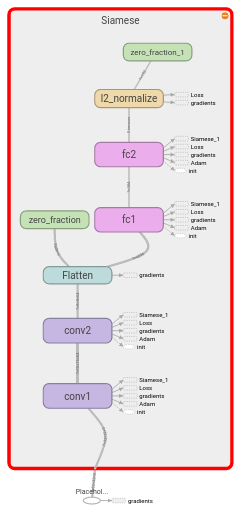
\includegraphics[width=.36\linewidth]{./images/model.png}
  \caption{Network}
  \label{fig:model}
\end{figure}

\subsection{Input}
The image features were obtained by passing images through the VGG net, pretained on ImageNet. The features correspond to the fifth convolutional layer. 

Attached to each image are five descriptive captions. Each caption consists of a single sentence. We processed this in order to create pairs of a single image and a single caption. All samples are seen by the network as independent from each other, thus enriching our datasets. 

%TODO: how do we feed this to the LSTM

\subsection{Vocabulary}
Words from the training captions are counted and stored. With Zipf's law in mind, we assume that low frequency words in our sample are also rare in the English language. Therefore, and to control for an extremely large vocabulary size, words with less than $n$ appearances in the total training set are discarded.

In the initial setup, we require a minimum of four appearances for a word to be kept in the vocabulary. Our reasoning is that if a word does not at least appear in all five captions of an image, then it is not essential for properly describing it. At the beginning, number of required appearances was chosen arbitrarily, however we experiment with different minimum and compare the effects it has on our results, but we analyze it further in section 5.

After counting and selecting the words to be included, we sort them by decreasing count, and store them for latter use.

\subsection{Word encoding}
Since the goal of this project is not to create optimal word embeddings, we encode words in the vocabulary in a basic way.
On a first instance, a word is encoded as its index in the vocabulary. Later we use one hot encoding and compare results. 

\subsubsection{Start/Stop tags} 
We create special codes for representing the start and end of a caption. This serves as mechanism to signal the network to stop generating words.

\section{Experimental setup}
The network was created using Theano and Lasagne.

\subsection{Data}
%TODO: check real sizes
The training set consists of 14,000 samples. The test set consists of 1,000 samples. Sample Images and their captions are shown in Figure \ref{fig:sample_input}

\begin{figure}[H]
  \centering
  
\includegraphics[width=.36\linewidth]{./images/sample_input.png}
  \caption{Sample image and its related descriptive caption.}
  \label{fig:sample_input}
\end{figure}

We perform batch training. 

\subsection{Training}

We train the implementation with the following parameters: 

%TODO: adapt table
\begin{tabular}{|c|c|}
\hline
\textbf{Parameter} & \textbf{Value}\\ \hline \hline
learning rate & 2e-3 \\ \hline
weight regularizer strength & 0. \\ \hline
weight initlaization scale & 1e-4 \\ \hline
batch size & 200 \\ \hline
maximum steps & 1500 \\ \hline
dropout rate & 0. \\ \hline
number of hidden neurons & '100' \\ \hline
type of weigh initialization & 'normal' \\ \hline
type of weight regularizer & 'l2' \\ \hline
activation function & 'relu' \\ \hline
optimizer & 'sgd' \\ \hline
loss & cross entropy \\ \hline
\end{tabular}

\subsection{Evaluation}
For evaluation we use the Baseline BLEU metric. According to Papineni et al \cite{papineni2002bleu}, it provides a quick, inexpensive and language independent method of evaluating machine translation, so it provides a good mechanism for us to evaluate our captions. In our system we are using the Natural Language Toolkit's (NLTK) implementation of the BLEU metric. Our captions are given a score between 0 and 1, where 1 means that the caption we generated was identical to our reference.

\begin{figure}[H]
	\centering
	\begin{subfigure}{\textwidth}
		\centering
		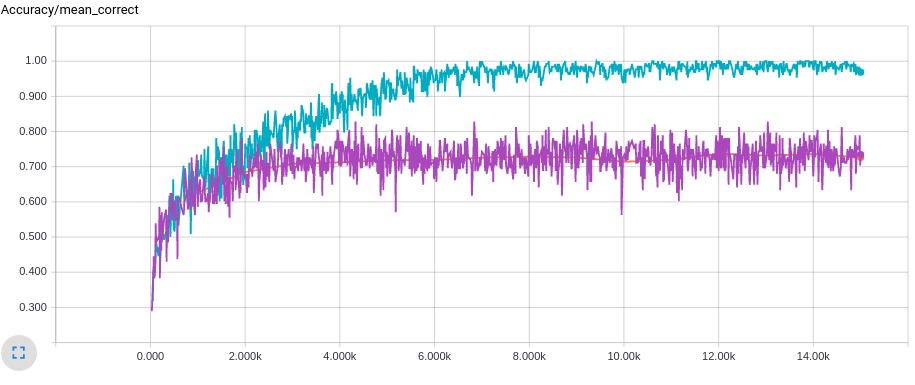
\includegraphics[width=0.75\linewidth]{./images/accuracy.png}
		\caption{BLUE scores here}
	\end{subfigure}
\end{figure}

\section{Results}
\subsection{Basic setup}

The model performance is shown in Figure \ref{fig:performance}

\begin{figure}[H]
  \centering
  \begin{subfigure}{\textwidth}
  	\centering
  	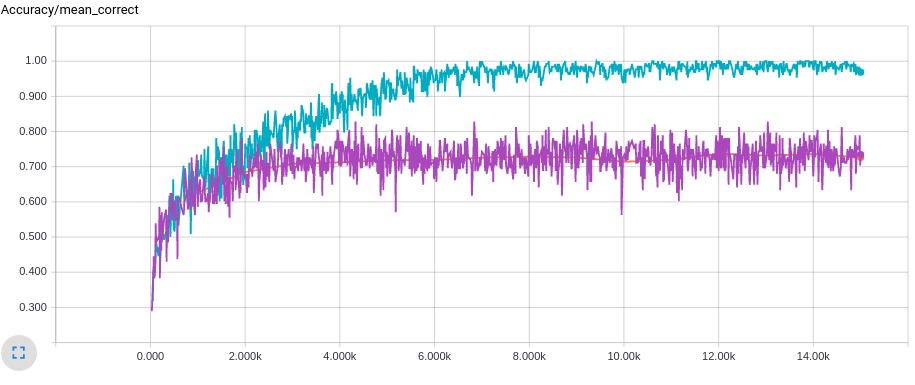
\includegraphics[width=0.75\linewidth]{./images/accuracy.png}
  	\caption{Accuracy}
  \end{subfigure}
  \begin{subfigure}{\textwidth}
  	\centering
  	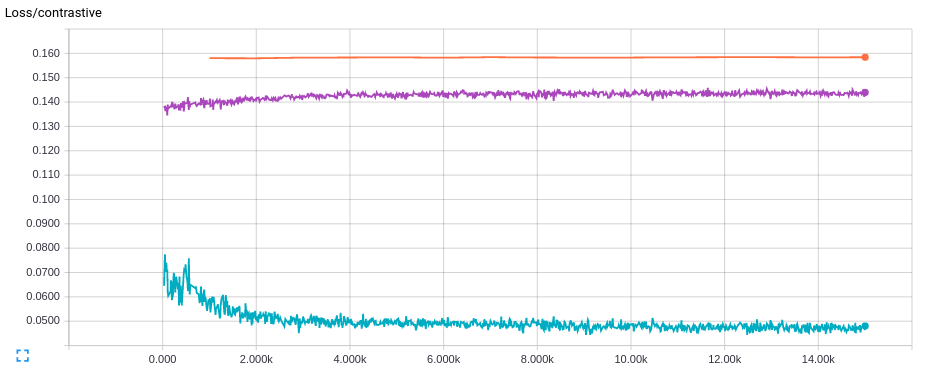
\includegraphics[width=0.75\linewidth]{./images/loss.png}
  	\caption{Loss}
  \end{subfigure}
  \caption{Performance for basic setup. Blue line corresponds to training, purple line corresponds to testing.}
  	\label{fig:performance}
\end{figure}

\subsection{Vocabulary size}
We test different minimum count values for including words in the vocabulary. This modules both the length of and diversity in our vocabulary.

\subsection{Word encoding}
We compare index encoding against one hot encoding.

\section{Conclusion}


\section*{References}

\small

[1] Abadi, M., Agarwal, A., Barham, P., Brevdo, E., Chen, Z., Citro, C., ... \ \& Ghemawat, S. \ (2015). TensorFlow: Large-scale machine learning on heterogeneous systems, 2015. {\it Software available from tensorflow. org}.


%TODO switch to sing bibliography, or unnecessary?? what is the others opinion?
\bibliographystyle{plain}
\bibliography{mybib}

\end{document}
